\documentclass[a4paper]{article}
\usepackage{graphicx}
\usepackage{amsmath}

\usepackage{geometry}
 \geometry{
 a4paper,
 total={150mm,257mm},
 top=20mm,
 }

\newcommand{\di}{i}
\begin{document}
\section{Edge current calculation}
Calculation of edge current, using trajectories from a point $(-L/2, y_i)$ at the left boundary through a fixed point $(x, y) = (0, \pm W/2)$ to a point at the right boundary $(+L/2, y_f)$. Assuming, trajectories are isotropically scattered from there to the right boundary with a transmission coefficient $\mathcal{T}_{\text{edge}}$.
\subsection{Upper edge}
Starting with the upper edge $(x, y) = (0, + W/2)$.
Parametrization of trajectory by angles $\theta_{i, f}$:
	\begin{eqnarray}
	\tan\theta_i = \frac{W - 2 y_i}{L}, \quad \frac{d \theta_i}{d y_i} = -\frac{2L}{L^2 + (W - 2y_i)^2}  \\
	\tan\theta_f =\frac{W - 2y_f}{L}, \quad  \frac{d \theta_f}{d y_f} = - \frac{2L}{L^2 + (W - 2 y_f)^2}.
	\end{eqnarray}	
Effective magnetic phase
	\begin{eqnarray}
	\frac{2\pi}{\Phi_0} \int d\mathbf{l} \cdot \mathbf{A}  &=& -\frac{2 \pi B}{\Phi_0} \left( \int_{-L/2}^{0} x \tan \theta_i dx + \int_{0}^{+L/2} x \tan \theta_f dx\right)\\
	&=& -\frac{\pi B}{\Phi_0} \left( \frac{L}{2}\right)^2 \left(\tan \theta_i + \tan \theta_f \right) \\
	&=& \frac{\pi \phi}{2 W} \left( y_i + y_f \right) + \frac{\pi \phi}{2} 
	\label{phase}
	\end{eqnarray}
First the critical current for zero flux, where we have no effective phase. Using the parametrization above and the current-phase relation
	\begin{equation}
	\mathcal{J}(\chi)\simeq  \mathcal{T} \sin\chi, \quad \mathcal{T}\ll 1,
	\label{sawT<1}
	\end{equation}
we find for zero magnetic field:
	\begin{eqnarray}
	I^{\text{edge}}_{c0} &=& \text{max}_{\chi} \int d \theta_i \cos^2 \theta_i\int d \theta_f \cos \theta_f \mathcal{J}(\chi)\\
	&=& \int_{-W/2}^{W/2} d y_i \frac{-2 L^3}{\left(L^2 + (W - 2y_i)^2\right)^2 }\int_{-W/2}^{W/2} dy_f \frac{-2 L^2}{\left(L^2 + (W - 2 y_f )^2 \right)^{3/2}}\\
	&=&  \frac{W}{\sqrt{L^2 + 4 W^2}} \arctan\left(\frac{2 W}{L} \right) + \frac{2 L W^2}{\left( L^2 + 4 W^2 \right)^{3/2}}.
	\label{ic0}
	\end{eqnarray}
For comparison the zero field critical current in the QPC setup is
	\begin{equation}
	I^{\text{qpc}}_{c0} =
	\frac{L}{\sqrt{L^2+W^2}}\arctan\frac{W}{L} + \frac{L^2W}{(L^2+W^2)^{3/2}}
	\label{Ic-0}
	\end{equation}	
Now with finite, but small magnetic flux $\phi$. Using the effective phase from eq. (\ref{phase}) for the Josephson relation in eq.(\ref{sawT<1}):
	\begin{eqnarray}
	\frac{I_c(\phi)}{I^{\text{edge}}_{c0}} &=& \frac{1}{I_{c0}} \text{max}_{\chi} \int d \theta_i \cos^2 \theta_i\int d \theta_f \cos \theta_f \mathcal{J}(\tilde{\chi}(y_i, y_f)) \\
	&=& 1 - \frac{\pi^2 \phi^2}{32}f_{\text{egde}}(W/L) \\
	f_{\text{egde}}(x) &=& 2 -\frac{\sqrt{4 x^2+1} -1}{x^2} - \frac{4 \left(2 x^2+1\right)}{2 x^2 + x\left(4 x^2+1\right) \arctan(2 x)} \\
	&\quad& - \frac{\sqrt{4 x^2+1} \log \left(\sqrt{4 x^2+1}-2 x\right)}{x^3}
	\end{eqnarray}
QPC function:
	\begin{eqnarray}
	\frac{I_c(\phi)}{I^{\text{qpc}}_{c0}}&\simeq& 1 - \frac{\pi ^2 \phi^2 }{32} f_0(W/L) \\
	f_0(x) &=& \frac{\sqrt{x^2+1} \log \left(\sqrt{x^2+1}+x\right)}{x}- \frac{x}{x+\left(x^2+1\right) \arctan(x)} 
	\end{eqnarray}
In the limit of high fields, extending the integration over $y_{i,f}$ to infinity, using $ \tilde{\phi} = \frac{\pi \phi}{2 W} $ we get ... \textit{to be completed} ...

%\begin{figure} 
%	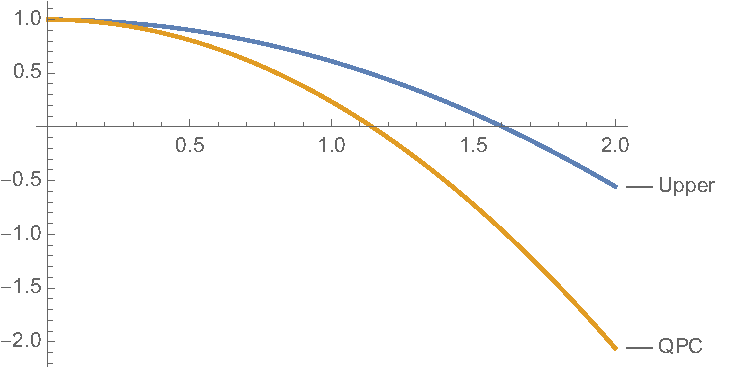
\includegraphics[width=0.8\textwidth]{plot_upper_qpc}
%\end{figure}	


\end{document}